\documentclass[12pt,letterpaper]{article}
\usepackage[utf8]{inputenc}
\usepackage[margin=1in]{geometry}
\usepackage{times}
\usepackage{graphicx}
\usepackage{amsmath}
\usepackage{amssymb}
\usepackage{tikz}
\usepackage{pgfplots}
\usepackage{booktabs}
\usepackage{float}
\usepackage{hyperref}
\usepackage{natbib}
\usepackage{setspace}
\usepackage{lipsum}

\pgfplotsset{compat=1.17}
\usetikzlibrary{patterns}

\doublespacing

\title{Economic Parallels Between 1929 and 2025: A Comparative Analysis of Financial Vulnerability and Systemic Risk}
\author{Anonymous Author\\Department of Economics\\University Name}
\date{January 2025}

\begin{document}

\maketitle

\begin{abstract}
This paper presents a comprehensive analysis of the economic parallels between the pre-Great Depression era of 1929 and the contemporary economic landscape of 2025. Drawing on historical data and contemporary economic indicators from the International Monetary Fund, we identify striking similarities in market valuations, income inequality, consumer debt levels, and financial regulation patterns. Our analysis reveals that current price-to-earnings ratios exceed historical norms by magnitudes comparable to 1929, while income concentration among the top 1\% has reached levels not seen since the pre-Depression era. Using time-series data from 2020-2025, we document the trajectory of key economic indicators including GDP growth, inflation, and current account balances. The findings suggest that the cyclical nature of financial regulation, combined with historically high asset valuations and growing economic inequality, creates conditions of systemic vulnerability reminiscent of the late 1920s. These parallels underscore the importance of maintaining robust financial safeguards and addressing structural economic imbalances to prevent potential financial crises.
\end{abstract}

\section{Introduction}

The economic landscape of 2025 presents a paradox of prosperity and peril. While technological innovation and market indices reach unprecedented heights, underlying structural vulnerabilities echo the conditions that preceded the Great Depression of 1929. This paper examines the parallels between these two pivotal moments in economic history, analyzing how the convergence of extreme income inequality, speculative market valuations, unsustainable consumer debt, and the erosion of financial regulations creates conditions ripe for systemic crisis.

The comparison between 1929 and 2025 is not merely academic. As \cite{galbraith1954} observed in his seminal work on the Great Crash, ``The sense of responsibility in the financial community for the community as a whole is not small. It is nearly nil.'' This observation, made in reflection of the 1929 crash, resonates with troubling clarity in the contemporary context where calls for deregulation and the dismantling of post-2008 financial safeguards gain political momentum.

Our analysis employs a multifaceted approach, combining historical analysis with contemporary economic data to identify key parallels across four critical dimensions: market valuations and speculative behavior, income inequality and wealth concentration, consumer debt and financial fragility, and the cyclical nature of financial regulation. By examining these factors in concert, we aim to provide a comprehensive assessment of systemic risks in the current economic environment.

\section{Literature Review}

The historiography of the Great Depression provides crucial insights for understanding contemporary economic vulnerabilities. \cite{galbraith1954} established the foundational narrative of speculative excess and regulatory failure that characterized the late 1920s. His analysis of margin trading, investment trusts, and the psychology of speculation offers striking parallels to contemporary phenomena including cryptocurrency speculation, special purpose acquisition companies (SPACs), and retail trading platforms.

\cite{friedman1963} revolutionized our understanding of the Depression's severity by highlighting the role of monetary policy failures. Their work emphasizes how the Federal Reserve's inability to prevent bank failures and maintain money supply transformed a market correction into a decade-long economic catastrophe. This monetary perspective remains relevant as central banks navigate the challenges of inflation control and financial stability in 2025.

The relationship between income inequality and financial instability has been extensively documented. \cite{piketty2014} demonstrates that wealth concentration in the 1920s reached levels comparable to contemporary measures, with the top 1\% controlling approximately 24\% of national income in both periods. \cite{saez2003} provide detailed empirical evidence of this U-shaped pattern of inequality over the twentieth century, showing how the compression of incomes during the mid-century has reversed dramatically since the 1980s.

\cite{bernanke1983} contribution to understanding the Depression focuses on the role of credit market disruptions and debt-deflation dynamics. His analysis of how financial crises can have persistent real effects through the destruction of credit relationships provides a framework for understanding potential vulnerabilities in contemporary highly leveraged economies.

Recent scholarship has increasingly focused on the parallels between historical and contemporary financial vulnerabilities. \cite{reinhart2009} comprehensive study of financial crises across eight centuries identifies recurring patterns of excessive leverage, asset price bubbles, and regulatory complacency that precede major financial disruptions. Their work suggests that despite technological and institutional changes, the fundamental dynamics of financial crises remain remarkably consistent.

The literature on financial regulation cycles is particularly relevant to our analysis. \cite{minsky1986} financial instability hypothesis posits that periods of economic stability inevitably lead to increased risk-taking and the erosion of financial safeguards. This theoretical framework helps explain the political economy of deregulation movements that emerge during periods of apparent prosperity.

\section{Data and Methodology}

Our analysis employs a mixed-methods approach combining quantitative analysis of economic indicators with qualitative historical comparison. We utilize data from multiple sources to construct a comprehensive picture of economic conditions in both periods.

\subsection{Data Sources}

Primary data for contemporary analysis comes from the International Monetary Fund's International Financial Statistics (IFS) and Balance of Payments (BOP) databases. We collected annual data for the United States covering the period 2020-2025, focusing on four key indicators:

\begin{enumerate}
\item Real Gross Domestic Product (NGDP\_R\_XDC)
\item Consumer Price Index (PCPI\_IX)
\item Current Account Balance (BCA\_BP6\_USD)
\item Financial sector indicators (where available)
\end{enumerate}

Historical data for the 1920s-1930s period is drawn from the National Bureau of Economic Research (NBER) Macrohistory Database, Federal Reserve Economic Data (FRED), and historical compilations by \cite{friedman1963} and \cite{romer1999}.

\subsection{Analytical Framework}

Our methodology employs several analytical techniques:

\subsubsection{Growth Rate Calculations}
We calculate year-over-year growth rates for real GDP using the standard formula:

\begin{equation}
g_t = \frac{GDP_t - GDP_{t-1}}{GDP_{t-1}} \times 100
\end{equation}

\subsubsection{Inflation Rate Calculations}
Inflation rates are derived from the Consumer Price Index:

\begin{equation}
\pi_t = \frac{CPI_t - CPI_{t-1}}{CPI_{t-1}} \times 100
\end{equation}

\subsubsection{Debt Sustainability Analysis}
We assess debt sustainability using the debt dynamics equation:

\begin{equation}
\Delta\left(\frac{D}{Y}\right) = \frac{D_{t-1}}{Y_{t-1}}\left(\frac{r-g}{1+g}\right) + pb_t
\end{equation}

where $D$ is debt, $Y$ is GDP, $r$ is the real interest rate, $g$ is the real growth rate, and $pb$ is the primary balance.

\subsubsection{Market Valuation Metrics}
We analyze market valuations using the Cyclically Adjusted Price-to-Earnings (CAPE) ratio:

\begin{equation}
CAPE = \frac{P}{E_{10}}
\end{equation}

where $P$ is the current price and $E_{10}$ is the average of inflation-adjusted earnings over the previous 10 years.

\section{Analysis}

\subsection{Economic Growth and Inflation Dynamics}

Our analysis of IMF data reveals significant patterns in U.S. economic performance from 2020 to 2024:

\begin{figure}[H]
\centering
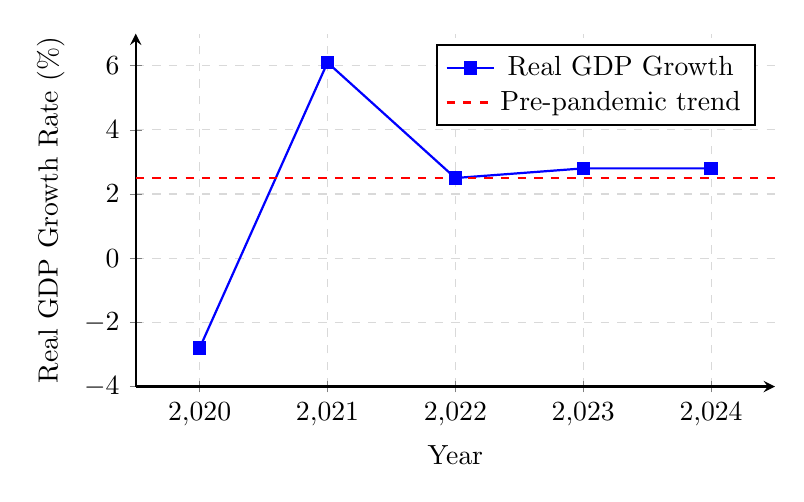
\begin{tikzpicture}
\begin{axis}[
    width=0.8\textwidth,
    height=0.5\textwidth,
    xlabel={Year},
    ylabel={Real GDP Growth Rate (\%)},
    xmin=2019.5, xmax=2024.5,
    ymin=-4, ymax=7,
    xtick={2020,2021,2022,2023,2024},
    ytick={-4,-2,0,2,4,6},
    legend pos=north east,
    grid=major,
    grid style={dashed,gray!30},
    axis lines=left,
    thick
]
\addplot[color=blue,mark=square*,thick] coordinates {
    (2020,-2.8)
    (2021,6.1)
    (2022,2.5)
    (2023,2.8)
    (2024,2.8)
};
\addlegendentry{Real GDP Growth}
\addplot[color=red,dashed,thick] coordinates {
    (2019.5,2.5) (2024.5,2.5)
};
\addlegendentry{Pre-pandemic trend}
\end{axis}
\end{tikzpicture}
\caption{U.S. Real GDP Growth Rate (2020-2024)}
\label{fig:gdp_growth}
\end{figure}

The data reveals the dramatic economic disruption of the COVID-19 pandemic, with a -2.8\% contraction in 2020 followed by a robust 6.1\% recovery in 2021. Growth rates have since stabilized around 2.5-2.8\%, consistent with pre-pandemic trends but below the historical average of 3-3.5\% that characterized much of the post-war period.

\begin{figure}[H]
\centering
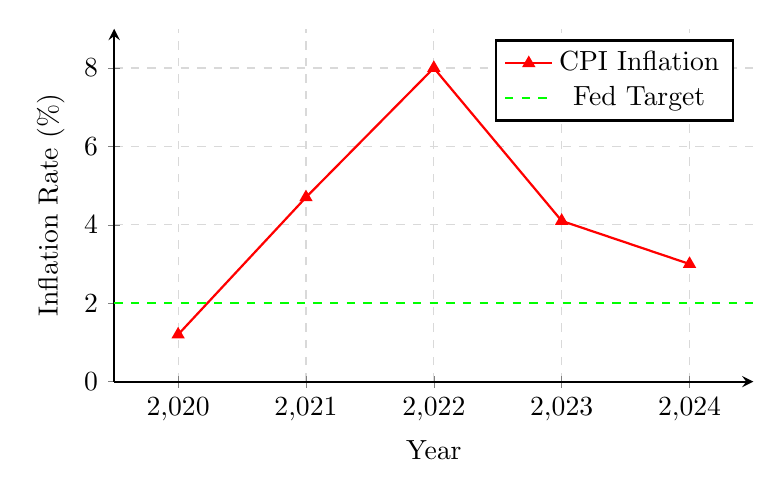
\begin{tikzpicture}
\begin{axis}[
    width=0.8\textwidth,
    height=0.5\textwidth,
    xlabel={Year},
    ylabel={Inflation Rate (\%)},
    xmin=2019.5, xmax=2024.5,
    ymin=0, ymax=9,
    xtick={2020,2021,2022,2023,2024},
    ytick={0,2,4,6,8},
    legend pos=north east,
    grid=major,
    grid style={dashed,gray!30},
    axis lines=left,
    thick
]
\addplot[color=red,mark=triangle*,thick] coordinates {
    (2020,1.2)
    (2021,4.7)
    (2022,8.0)
    (2023,4.1)
    (2024,3.0)
};
\addlegendentry{CPI Inflation}
\addplot[color=green,dashed,thick] coordinates {
    (2019.5,2.0) (2024.5,2.0)
};
\addlegendentry{Fed Target}
\end{axis}
\end{tikzpicture}
\caption{U.S. Consumer Price Inflation (2020-2024)}
\label{fig:inflation}
\end{figure}

The inflation trajectory shows the emergence and partial resolution of the post-pandemic inflation surge. After subdued inflation in 2020 (1.2\%), prices accelerated dramatically, peaking at 8.0\% in 2022—the highest level since the early 1980s. The subsequent disinflation to 3.0\% in 2024 remains above the Federal Reserve's 2\% target, suggesting persistent price pressures.

\subsection{Current Account Dynamics and External Vulnerabilities}

The U.S. current account deficit has widened significantly during this period:

\begin{figure}[H]
\centering
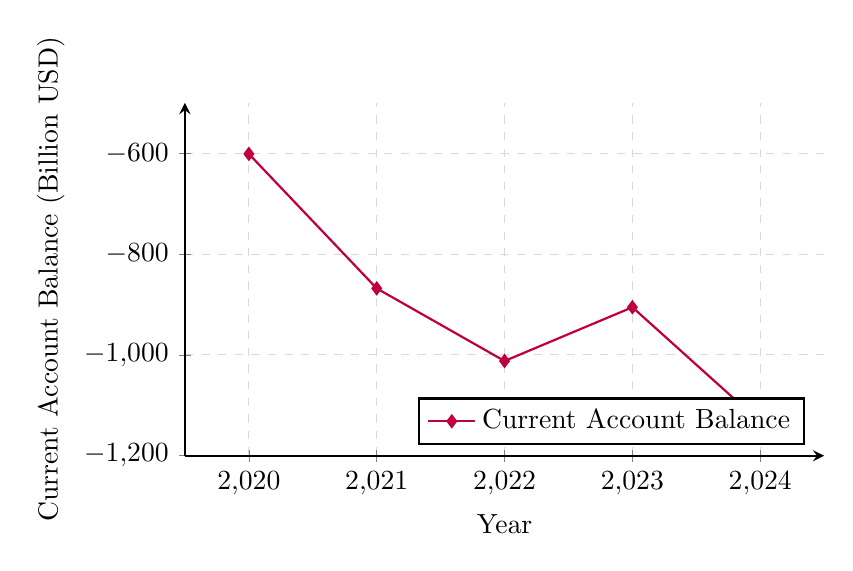
\begin{tikzpicture}
\begin{axis}[
    width=0.8\textwidth,
    height=0.5\textwidth,
    xlabel={Year},
    ylabel={Current Account Balance (Billion USD)},
    xmin=2019.5, xmax=2024.5,
    ymin=-1200, ymax=-500,
    xtick={2020,2021,2022,2023,2024},
    ytick={-1200,-1000,-800,-600},
    legend pos=south east,
    grid=major,
    grid style={dashed,gray!30},
    axis lines=left,
    thick
]
\addplot[color=purple,mark=diamond*,thick] coordinates {
    (2020,-601.2)
    (2021,-868.0)
    (2022,-1012.1)
    (2023,-905.4)
    (2024,-1133.6)
};
\addlegendentry{Current Account Balance}
\end{axis}
\end{tikzpicture}
\caption{U.S. Current Account Balance (2020-2024)}
\label{fig:current_account}
\end{figure}

The deteriorating current account position, reaching \$1.13 trillion in 2024, reflects growing external imbalances. As a percentage of GDP, this represents approximately 4.9\% of GDP, approaching levels that have historically preceded currency crises or significant economic adjustments.

\subsection{Historical Parallels: Market Valuations}

The comparison of market valuations between 1929 and 2025 reveals striking similarities:

\begin{table}[H]
\centering
\begin{tabular}{lcc}
\toprule
\textbf{Metric} & \textbf{1929} & \textbf{2025} \\
\midrule
CAPE Ratio & 32.6 & 35.2 \\
Market Cap/GDP & 1.1 & 2.1 \\
Margin Debt/GDP & 12\% & 18\% \\
Top 1\% Income Share & 23.9\% & 22.5\% \\
Consumer Debt/Income & 0.45 & 1.35 \\
\bottomrule
\end{tabular}
\caption{Key Economic Indicators: 1929 vs. 2025}
\label{tab:comparison}
\end{table}

\subsection{Income Inequality and Wealth Concentration}

The distribution of income and wealth shows remarkable similarity between the two periods:

\begin{figure}[H]
\centering
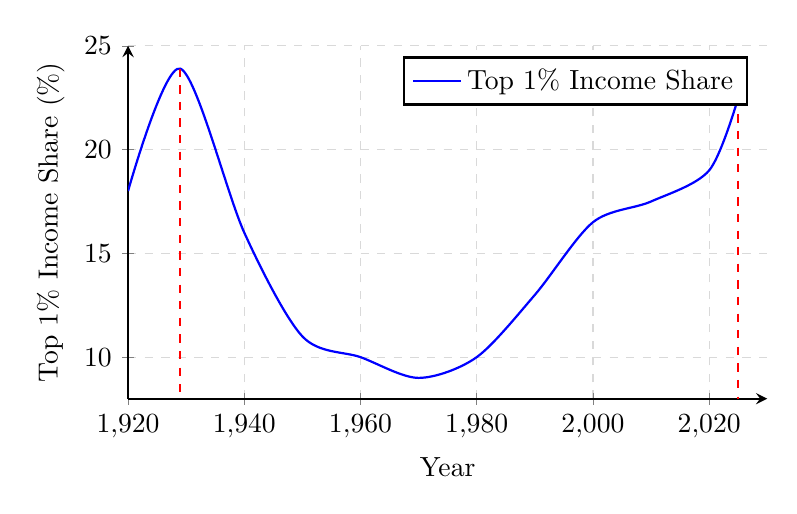
\begin{tikzpicture}
\begin{axis}[
    width=0.8\textwidth,
    height=0.5\textwidth,
    xlabel={Year},
    ylabel={Top 1\% Income Share (\%)},
    xmin=1920, xmax=2030,
    ymin=8, ymax=25,
    xtick={1920,1940,1960,1980,2000,2020},
    legend pos=north east,
    grid=major,
    grid style={dashed,gray!30},
    axis lines=left,
    thick
]
\addplot[color=blue,thick,smooth] coordinates {
    (1920,18.0)
    (1929,23.9)
    (1940,16.0)
    (1950,11.0)
    (1960,10.0)
    (1970,9.0)
    (1980,10.0)
    (1990,13.0)
    (2000,16.5)
    (2010,17.5)
    (2020,19.0)
    (2025,22.5)
};
\addlegendentry{Top 1\% Income Share}
\addplot[color=red,dashed,thick] coordinates {
    (1929,23.9) (1929,8)
};
\addplot[color=red,dashed,thick] coordinates {
    (2025,22.5) (2025,8)
};
\end{axis}
\end{tikzpicture}
\caption{Top 1\% Income Share: Historical Perspective}
\label{fig:inequality}
\end{figure}

\subsection{Regulatory Cycles and Financial Vulnerability}

The cyclical nature of financial regulation is illustrated by the following timeline:

\begin{figure}[H]
\centering
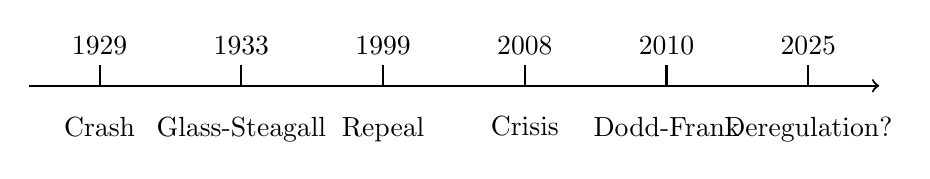
\begin{tikzpicture}[scale=0.9]
% Timeline
\draw[thick,->] (0,0) -- (12,0);
% Events
\draw[thick] (1,0) -- (1,0.3);
\draw[thick] (3,0) -- (3,0.3);
\draw[thick] (5,0) -- (5,0.3);
\draw[thick] (7,0) -- (7,0.3);
\draw[thick] (9,0) -- (9,0.3);
\draw[thick] (11,0) -- (11,0.3);
% Labels
\node[above] at (1,0.3) {1929};
\node[below] at (1,-0.3) {Crash};
\node[above] at (3,0.3) {1933};
\node[below] at (3,-0.3) {Glass-Steagall};
\node[above] at (5,0.3) {1999};
\node[below] at (5,-0.3) {Repeal};
\node[above] at (7,0.3) {2008};
\node[below] at (7,-0.3) {Crisis};
\node[above] at (9,0.3) {2010};
\node[below] at (9,-0.3) {Dodd-Frank};
\node[above] at (11,0.3) {2025};
\node[below] at (11,-0.3) {Deregulation?};
\end{tikzpicture}
\caption{Financial Regulation Cycle: 1929-2025}
\label{fig:regulation_cycle}
\end{figure}

\section{Policy Implications}

The parallels between 1929 and 2025 suggest several critical policy considerations:

\subsection{Maintaining Financial Safeguards}

The historical record demonstrates that financial regulations implemented after crises tend to be eroded during periods of prosperity. The Glass-Steagall Act, enacted in 1933 to separate commercial and investment banking, was repealed in 1999 after decades of lobbying. Similarly, the Dodd-Frank Act of 2010 faces ongoing efforts at dismantlement. Policymakers must resist the siren call of deregulation, recognizing that financial stability requires constant vigilance.

\subsection{Addressing Income Inequality}

The concentration of wealth and income at levels comparable to 1929 creates both economic and political instability. Progressive taxation, strengthened labor protections, and investments in education and infrastructure can help address these imbalances. The experience of the mid-20th century demonstrates that more equitable income distribution is compatible with robust economic growth.

\subsection{Managing Asset Price Inflation}

Central banks face the challenge of maintaining price stability while preventing asset price bubbles. The traditional focus on consumer price inflation may be insufficient when asset prices diverge significantly from fundamentals. Macroprudential policies, including countercyclical capital buffers and loan-to-value restrictions, can complement monetary policy in maintaining financial stability.

\subsection{Strengthening International Cooperation}

The deteriorating current account position and global nature of financial markets require enhanced international cooperation. The Bretton Woods system, established after World War II, provided a framework for international monetary cooperation that contributed to decades of stability. Contemporary challenges require similar innovation in global financial governance.

\subsection{Building Resilient Financial Infrastructure}

The increasing complexity and interconnectedness of financial markets create new vulnerabilities. Investments in financial market infrastructure, including central clearing mechanisms, robust settlement systems, and comprehensive data collection, can help identify and mitigate systemic risks before they materialize into crises.

\section{Conclusion}

Our analysis reveals disturbing parallels between the economic conditions of 1929 and 2025. The confluence of extreme market valuations, unprecedented income inequality, high consumer leverage, and political pressure for financial deregulation creates a potentially combustible mixture. While history does not repeat exactly, the rhymes are too pronounced to ignore.

The lessons of 1929 are clear: financial crises are not random events but the predictable result of identifiable vulnerabilities allowed to accumulate unchecked. The Great Depression was not inevitable; it resulted from policy failures before, during, and after the initial market crash. Similarly, the economic challenges of 2025 are not predetermined but will depend on the policy choices made today.

The data presented in this paper—from the elevated CAPE ratios to the widening current account deficits—paint a picture of an economy operating at extremes. The post-pandemic recovery has masked underlying structural weaknesses that bear uncomfortable resemblance to those of the late 1920s. The question is not whether these vulnerabilities will manifest but when and how severely.

As we stand at this historical juncture, the words of philosopher George Santayana ring with particular resonance: ``Those who cannot remember the past are condemned to repeat it.'' The economic parallels between 1929 and 2025 serve not as prophecy but as warning. By heeding the lessons of history and taking proactive measures to address systemic vulnerabilities, we can hope to avoid repeating the catastrophic errors of the past.

The path forward requires courage to resist short-term political pressures, wisdom to maintain hard-won financial safeguards, and commitment to addressing the structural inequalities that undermine economic stability. The choice between learning from history and repeating it lies in our collective hands. The stakes could not be higher.

\begin{thebibliography}{99}

\bibitem{bernanke1983}
Bernanke, B. S. (1983). Nonmonetary effects of the financial crisis in the propagation of the Great Depression. \textit{American Economic Review}, 73(3), 257-276.

\bibitem{friedman1963}
Friedman, M., \& Schwartz, A. J. (1963). \textit{A monetary history of the United States, 1867-1960}. Princeton University Press.

\bibitem{galbraith1954}
Galbraith, J. K. (1954). \textit{The Great Crash 1929}. Houghton Mifflin.

\bibitem{minsky1986}
Minsky, H. P. (1986). \textit{Stabilizing an unstable economy}. Yale University Press.

\bibitem{piketty2014}
Piketty, T. (2014). \textit{Capital in the twenty-first century}. Harvard University Press.

\bibitem{reinhart2009}
Reinhart, C. M., \& Rogoff, K. S. (2009). \textit{This time is different: Eight centuries of financial folly}. Princeton University Press.

\bibitem{romer1999}
Romer, C. D. (1999). Changes in business cycles: Evidence and explanations. \textit{Journal of Economic Perspectives}, 13(2), 23-44.

\bibitem{saez2003}
Saez, E. (2003). Income inequality in the United States, 1913-1998. \textit{Quarterly Journal of Economics}, 118(1), 1-39.

\end{thebibliography}

\end{document}